%% This is the main file and you use this file to organize your assignment. 

\documentclass[12pt,a4paper]{article}	  % Fontsize 12 pt.
\usepackage[margin=3cm]{geometry} 	   % Choose your margin here. 
\usepackage{amsmath}
\usepackage{parskip}
\usepackage{graphicx}
\usepackage{caption}
\usepackage{subcaption}
\usepackage{cancel}


\newcommand{\figref}[1]{\figurename~\ref{#1}}

\let\endtitlepage\relax						% Begin the text immidiately after the title page. Optional
\setlength{\parindent}{0cm}				% Start paragraph without indent. Optional

\begin{document}

\begin{titlepage}
\begin{center}
\Large TTK4190 Guidance and Control of Vehicles \\
\vspace{10pt}
\Large Assignment 1 \\
\vspace{10pt}
\large September 2016 \\By Magnus Aarskog
\end{center}
\end{titlepage}




\section*{Problem 1 - Attitude Kinematics and Kinetics}

\subsection*{Problem 1.1} 
\subsubsection*{1. Euler angles}
In \cite{Fossen2011} Euler angles and body-fixed angular velocity are written as
\begin{equation}\label{eq:using}
    \mathbf{\Theta}_{nb} = 
    \begin{bmatrix}
    \phi \\ \theta \\ \psi
    \end{bmatrix}
    \quad
    \text{and}
    \quad
    \boldsymbol{\omega}_{b/n}^b =
    \begin{bmatrix}
   p \\ q \\ r
    \end{bmatrix}
\end{equation}

Using equation (2.26) and (2.28) in \cite{Fossen2011} and equation (\ref{eq:using}) we get
\begin{equation}\label{eq:see}
    \dot{\mathbf{\Theta}}_{nb} = \mathbf{T}_\Theta (\mathbf{\Theta}_{nb})\boldsymbol{\omega}_{b/n}^b
     = 
     \begin{bmatrix}
     1 & s\phi t\theta & c\phi t\theta \\
     0 & c\phi & -s\phi \\
     0 & \frac{s\phi}{c\theta} & \frac{c\phi}{c\theta}
     \end{bmatrix}
    \begin{bmatrix}
   p \\ q \\ r
    \end{bmatrix}
\end{equation}
we can see from equation (\ref{eq:see}) that $\mathbf{Q} = \mathbf{T}_\Theta (\mathbf{\Theta}_{nb})$ and $\mathbf{T}(\boldsymbol{Q,\omega}) = \mathbf{T}_\Theta (\mathbf{\Theta}_{nb})\boldsymbol{\omega}_{b/n}^b$







\subsubsection*{2. Unit quaternions}

In equation (2.54) in \cite{Fossen2011} the unit quaternions are expressed in the form 
\begin{equation}
    \mathbf{q}=
    \begin{bmatrix}
        \eta \\ \varepsilon_1 \\ \varepsilon_2 \\ \varepsilon_3
    \end{bmatrix}
    =
    \begin{bmatrix}
            \cos\left(\frac{\beta}{2}\right) \\ \boldsymbol{\lambda} \sin\left(\frac{\beta}{2}\right)
    \end{bmatrix}
    , \quad \boldsymbol{\lambda} = \pm \frac{\boldsymbol{\varepsilon}}{\sqrt{\boldsymbol{\varepsilon}^T\boldsymbol{\varepsilon}}}, \quad 0 \le \beta \le 2\pi
\end{equation}

Again we look in \cite{Fossen2011} at equation (2.62) and (2.63) and we get the angular velocity transformation
\begin{equation}\label{eq:see2}
    \dot{\boldsymbol{q}} = \boldsymbol{T}_q(\boldsymbol{q})\boldsymbol{\omega}_{b/n}^b
    = \frac{1}{2}
    \begin{bmatrix}
    -\varepsilon_1 & -\varepsilon_2 & -\varepsilon_3\\
    \eta & -\varepsilon_3 & \varepsilon_2 \\
    \varepsilon_3 & \eta & -\varepsilon_1 \\
    -\varepsilon_2 & \varepsilon_1 & \eta
    \end{bmatrix}
    \begin{bmatrix}
   p \\ q \\ r
    \end{bmatrix}
\end{equation}
From equation (\ref{eq:see2}) we see that $\boldsymbol{Q} =\boldsymbol{T}_q(\boldsymbol{q})$ and $\mathbf{T}(\boldsymbol{Q,\omega}) = \boldsymbol{T}_q(\boldsymbol{q})\boldsymbol{\omega}_{b/n}^b$ 







\subsubsection*{3. Rotation matrix}
Equation (2.33) in \cite{Fossen2011} gives
\begin{equation}
    \dot{\boldsymbol{R}}_n^b = \boldsymbol{R}_n^b\boldsymbol{S(\boldsymbol{\omega}_{b/n}^b)}
\end{equation}
where $\boldsymbol{R}_n^b(\boldsymbol{\Theta}_{nb})$ are the product of the three principal rotations: $\boldsymbol{R}_n^b = \boldsymbol{R}_{z,\psi}\boldsymbol{R}_{y,\theta}\boldsymbol{R}_{x,\phi}$. From this we get $\boldsymbol{Q} = \boldsymbol{R}_n^b$ and $\boldsymbol{T}(\boldsymbol{Q},\boldsymbol{\omega}) = \boldsymbol{R}_n^b\boldsymbol{S(\boldsymbol{\omega}_{b/n}^b)}$







\subsection*{Problem 1.2}
\subsubsection*{Euler angles}
When using Euler angles, $\boldsymbol{Q}$ is not defined for $\theta = 90^\circ$. This is very unwanted since we are trying to control a satellite. Euler angles are intuitive to understand. 

\subsubsection*{Quaternions}
Here we don't have the same problem as with Euler angles when $\theta = 90^o$, but we have 4 parameters. Quaternions are more complicated to understand.  Quaternions are more stable and computationally faster. It is possible to make smooth rotations. 
\subsubsection*{Rotation matrix}
If a rotation matrix is used we will get 9 differential equations this means that it can be more difficult to compute. Round-off errors accumulate. 

\subsection*{Problem 1.3}
If the inertial frame is always below the satellite the Newton Euler EOM will be:\\From eq. (3.21) in \cite{Fossen2011}
\begin{equation}
    \begin{bmatrix}
        m\boldsymbol{I}_{3\text{x}3} & \boldsymbol{0}_{3\text{x}3}\\
        \boldsymbol{0}_{3\text{x}3} & \boldsymbol{I}_g
    \end{bmatrix}
    \begin{bmatrix}
        \boldsymbol{0} \\ \dot{\boldsymbol{\omega}}_{b/n}^b
    \end{bmatrix}
    +
    \begin{bmatrix}
        m\boldsymbol{S}(\boldsymbol{\omega}_{b/n}^b) &  \boldsymbol{0}_{3\text{x}3} \\
         \boldsymbol{0}_{3\text{x}3} & -\boldsymbol{S}(\boldsymbol{I}_g\boldsymbol{\omega}_{b/n}^b)
    \end{bmatrix}
        \begin{bmatrix}
        \boldsymbol{0} \\ \boldsymbol{\omega}_{b/n}^b
    \end{bmatrix}
    =
    \begin{bmatrix}
    \boldsymbol{f}_g^b \\ \boldsymbol{m}_g^b
    \end{bmatrix}
\end{equation}

This means the translational part of the equations are zero and the remaining equation is
\begin{subequation}
\begin{equation}
    \boldsymbol{I}_g\dot{\boldsymbol{\omega}}_{b/n}^b -\boldsymbol{S}(\boldsymbol{I}_g\boldsymbol{\omega}_{b/n}^b)\boldsymbol{\omega}_{b/n}^b = \boldsymbol{m}_g^b
\end{equation}
which is the same as 
\begin{equation}
	\label{eq:kinetics}
	\boldsymbol{I}_{CG} \dot{\boldsymbol{\omega}} - (\boldsymbol{I}_{CG} \boldsymbol{\omega}) \times \boldsymbol{\omega} = \boldsymbol{\tau}                                                                 
\end{equation}
\end{subequation}


which is the equation we wanted.

% Note that \mathbf can be used for bold letters in math mode (within equations and dollar signs). \boldsymbol is used to get bold greek letters.  	% Use "\include" instead of "\input" if you want the section to start on a new page. "problem1" is a tex file included at this location in the document. It is possible to answer the whole assignment in this file (paste everything from "problem1.tex" here), but that restricts the readability. Therefore, one file is created for each problem.
\section*{Problem 2 - Attitude Control using Euler Angles}
\subsection*{Problem 2.1}
The Lyapunov function candidate and the PD-controller can be written as 

\begin{equation}
\begin{aligned}\label{eq:yes}
	V &= \frac{1}{2} \boldsymbol{\omega}^{\top} \mathbf{I}_{CG} \boldsymbol{\omega} + \frac{1}{2} \tilde{\Theta}^{\top} \mathbf{K}_p \tilde{\Theta} \\
	\boldsymbol{\tau} &= -\mathbf{K}_d \boldsymbol{\omega} -\mathbf{T}_{\Theta}^{\top}(\Theta) \mathbf{K}_p \tilde{\Theta}
\end{aligned}
\end{equation}


Since $\boldsymbol{I}_{CG}$, $\boldsymbol{K}_d$ and $\boldsymbol{K}_p$ are symmetric, $\dot{V}$ becomes
\begin{equation} \label{eq:as}
\dot{V} = \boldsymbol{\omega}^T\boldsymbol{I}_{CG}\dot{\boldsymbol{\omega}} + \tilde{\Theta}^T\boldsymbol{K}_p\dot{\Theta}
\end{equation}

Inserting  (\ref{eq:kinetics}) into (\ref{eq:as})

\begin{equation}
\dot{V} = \boldsymbol{\omega}^T\left( \tau + (\boldsymbol{I}_{CG}\boldsymbol{\omega})\times \omega \right)
\end{equation}

\subsection*{Problem 2.2}
Answer Problem 2.2 here.

\subsection*{Problem 2.3}
Answer Problem 2.3 here.

\subsection*{Problem 2.4}
Answer Problem 2.4 here. Figures can be inserted as:
\begin{figure}[ht]
	\centering
	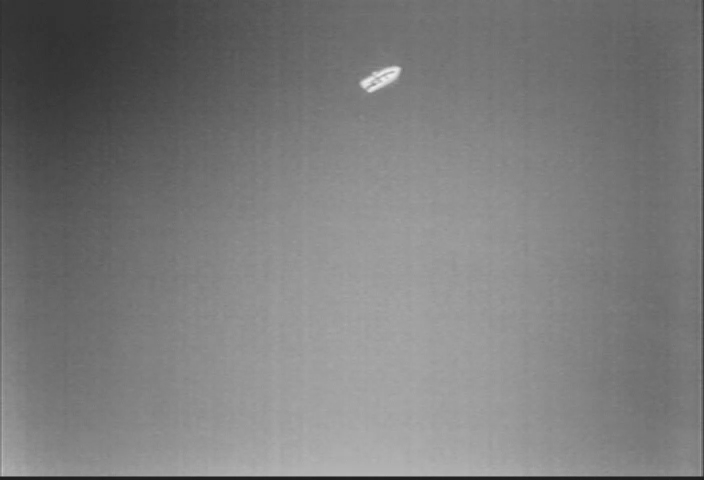
\includegraphics[width=0.7\textwidth]{fig1} % Filename is "fig1.png" and must be located in the same folder as this file. 
	\caption{Figure of something useful.}
	\label{fig:fig1}
\end{figure}

You can now refer to this figure as \figref{fig:fig1}. You can also insert figures side-by-side:
\begin{figure}[ht]
	\centering
	\begin{subfigure}[b]{0.45\textwidth}
		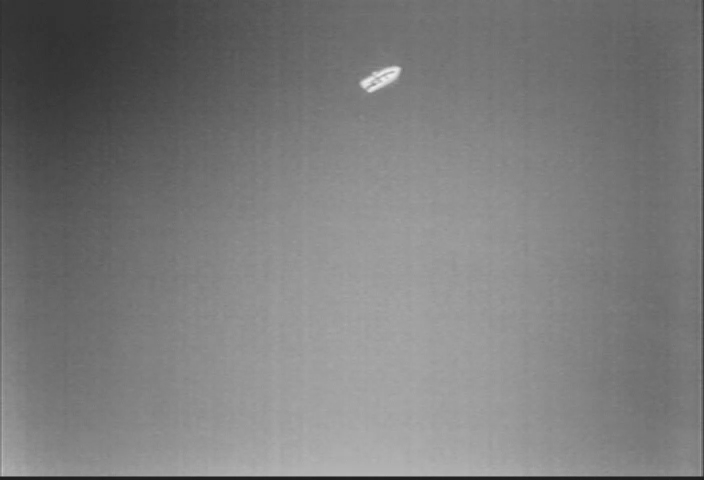
\includegraphics[width=\textwidth]{fig1}
		\caption{Fig 2a)}
		\label{fig:2a}
	\end{subfigure}
	~ %add desired spacing between images, e. g. ~, \quad, \qquad, \hfill etc. 
	%(or a blank line to force the subfigure onto a new line)
	\begin{subfigure}[b]{0.45\textwidth}
		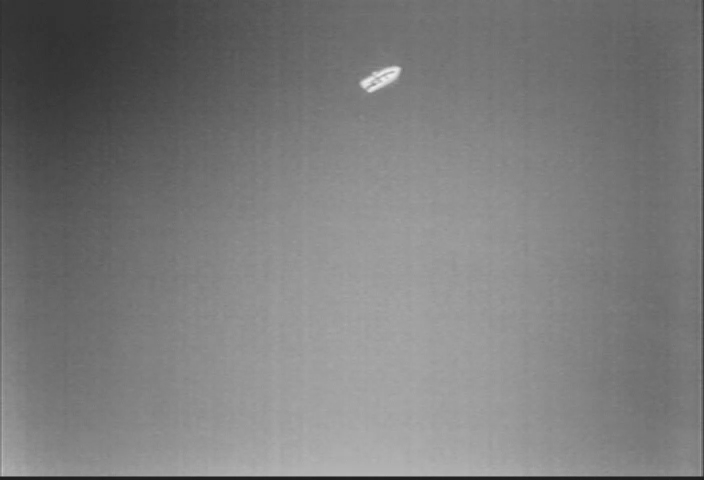
\includegraphics[width=\textwidth]{fig1}
		\caption{Fig 2b)}
		\label{fig:2b}
	\end{subfigure}
	\caption{Caption for both figures}\label{fig:2}
\end{figure}
\section*{Problem 3 - Attitude Control using Unit Quaternions}
Answer Problem 3 in this file.

\subsection*{Problem 3.1}
Answer Problem 3.1 here. The definition of the quaternion error is written as:
\begin{equation}
\tilde{\mathbf{q}} = \begin{bmatrix} \tilde{\eta} \\ \tilde{\boldsymbol{\epsilon}} \end{bmatrix} =\overline{\mathbf{q}_d} \otimes \mathbf{q}
\end{equation}

\subsection*{Problem 3.2}
Answer Problem 3.2 here. If you want to make a reference to the book, you can do that with the cite command: \cite{Fossen2011}. The data for the references must be created in the "bibliography.bib" file. The other references in the assignment are also stored in the bibliography. Cite them as \cite{Chateurverdi} and \cite{Fjellstad1994857}. Note that you need to install BibTeX to compile the bibliography.

\subsection*{Problem 3.3}
Answer Problem 3.3 here.

\section*{Problem 4 - Attitude Control using Rotation matrices}
 Answer Problem 4 in this file.
 
\subsection*{Problem 4.1}
Answer Problem 4.1 here. The map $\boldsymbol{\Omega}_{\mathbf{a}}(\mathbf{R})$ can be written in \LaTeX{} as:
\begin{equation}
\boldsymbol{\Omega}_{\mathbf{a}}(\mathbf{R}) := \sum \limits_{i=1}^3 a_i \mathbf{e}_i \times (\mathbf{R}_d^{\top} \mathbf{R} \mathbf{e}_i)
\end{equation} 

\subsection*{Problem 4.2}
Answer problem 4.2 here.

\subsection*{Problem 4.3}
Answer problem 4.3 here.
 
 https://en.wikipedia.org/wiki/Quaternions_and_spatial_rotation#Comparison_with_other_representations_of_rotations
 
\bibliographystyle{IEEEtran}
\bibliography{bibliography.bib}

\end{document}